\chapter{The Poisson distribution}
\label{ch:poisson}

\textbf{\underline{Example~1}}\medskip

A \emph{declustered} earthquake catalog\footnote{Mueller, C.S.,
  2019. Earthquake catalogs for the USGS national seismic hazard
  maps. \textit{Seismological Research Letters}, 90(1), pp.251-261.}
of the western United States contains 543 events of magnitude 5.0 and
greater that occurred between 1917 and 2016:\medskip

\noindent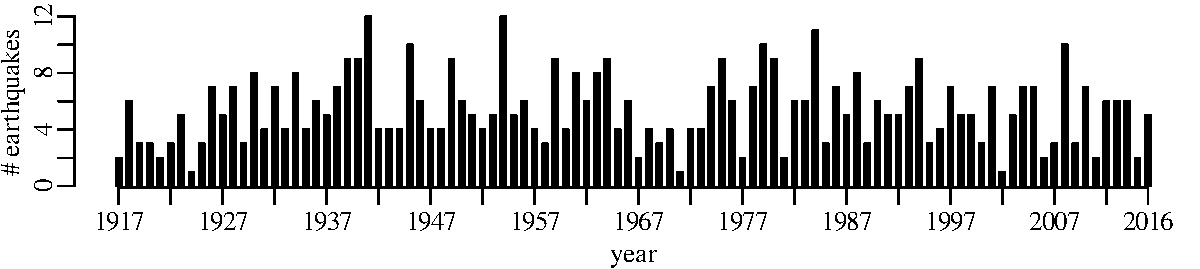
\includegraphics[width=\textwidth]{../figures/declusteredquakes.pdf}
\begingroup \captionof{figure}{The number of US earthquakes of
  magnitude 5.0 or greater per year between 1917 and 2016, with
  aftershocks removed.\medskip}
\label{fig:declusteredquakes}
\endgroup

The number of earthquakes in each bin forms a new dataset of 100
numbers, which has the following summary statistics:

\noindent\begin{minipage}[t][][b]{.4\textwidth}
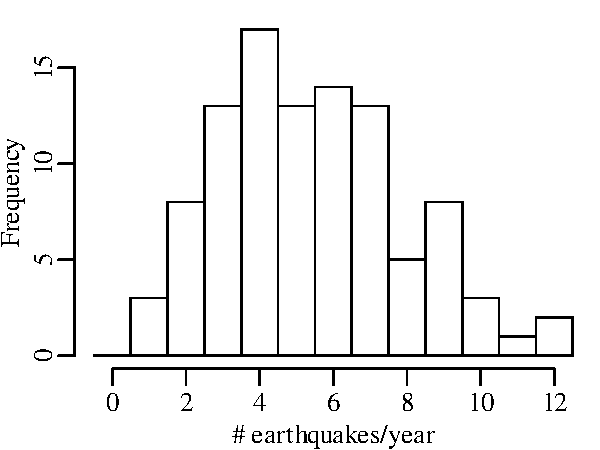
\includegraphics[width=\textwidth]{../figures/declusteredquakesperyear.pdf}
\medskip
\end{minipage}
\begin{minipage}[t][][t]{.6\textwidth}
  \captionof{figure}{ Histogram of the earthquake counts shown in
    Figure~\ref{fig:declusteredquakes}.\medskip
    ~\\
    \textbf{mean: 5.43}\\
    standard deviation: 2.50\\
    \textbf{variance: 6.24}
  }
  \label{fig:declusteredquakesperyear}
\end{minipage}

Note how the mean and the variance of this dataset are similar.\medskip

\noindent\textbf{\underline{Example~2}}\medskip

5000 grains of sand have been mounted in an uncovered thin section and
imaged with a scanning electron microscope (SEM). The SEM has
identified the locations of zircon (ZrSiO\textsubscript{4}) crystals
that are suitable for geochronological dating:

\noindent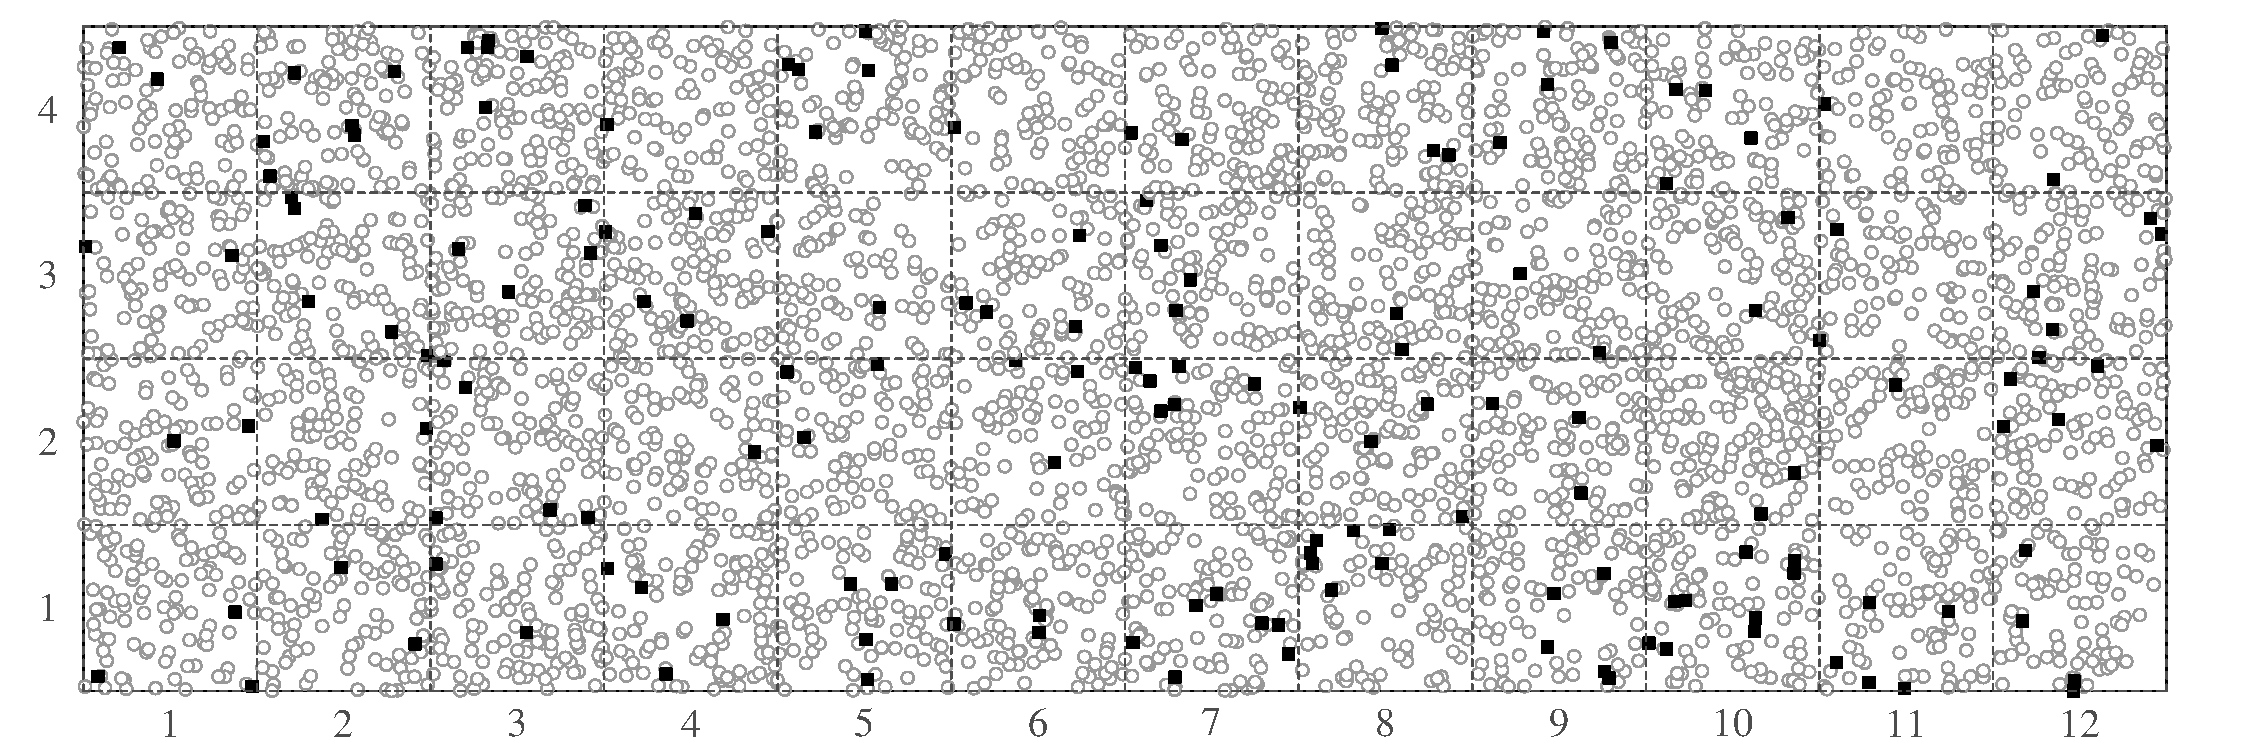
\includegraphics[width=\textwidth]{../figures/zircons.pdf}
\begingroup \captionof{figure}{Point-counting results for zircon in
  sand. Black squares mark zircons and grey circles other minerals.\medskip}
\label{fig:zircons}
\endgroup

Counting the number of zircons in the graticule:

\noindent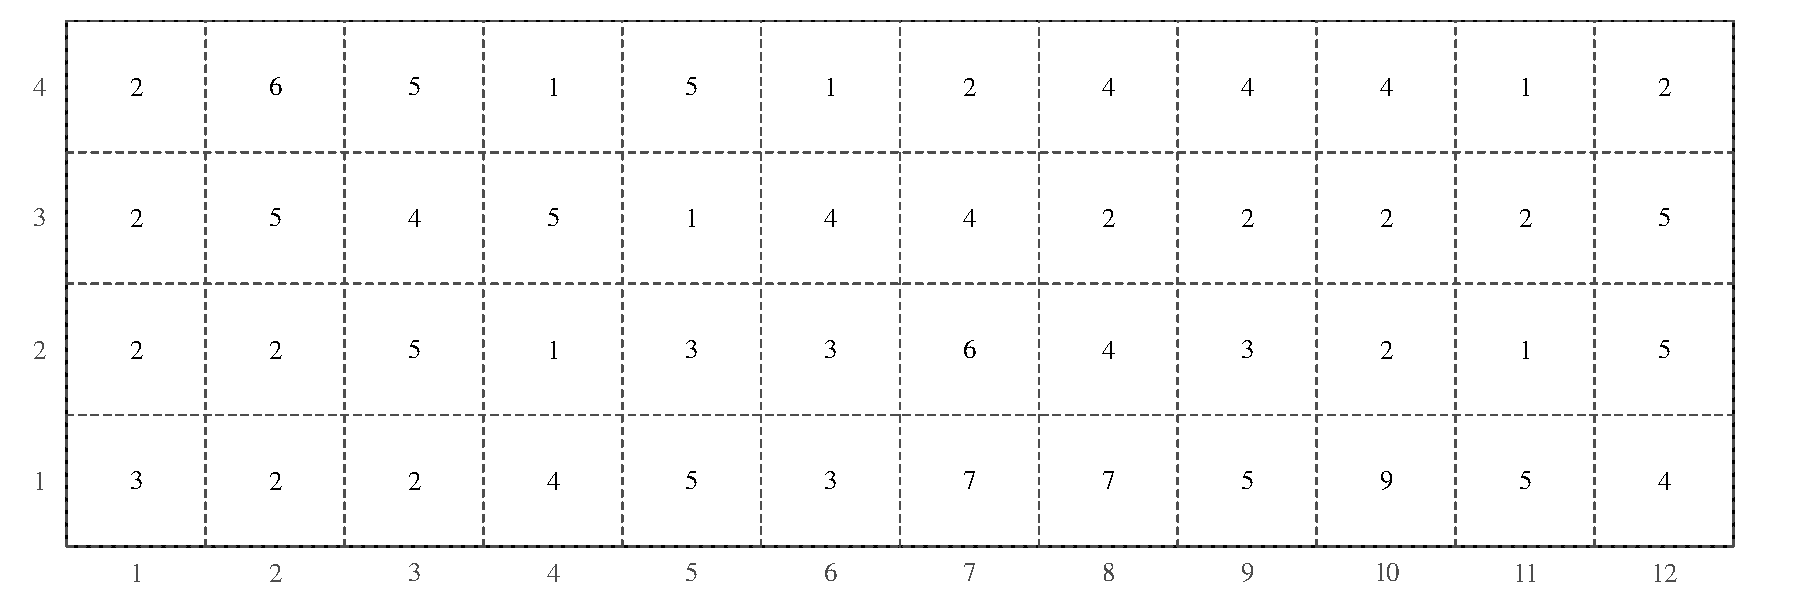
\includegraphics[width=\textwidth]{../figures/zirconcounts.pdf}
\begingroup \captionof{figure}{The number of zircons counted in each
  square of Figure~\ref{fig:zircons}.\medskip}
\label{fig:zirconcounts}\endgroup

And tallying the number of zircons per square in a histogram:

\noindent\begin{minipage}[t][][b]{.3\textwidth}
  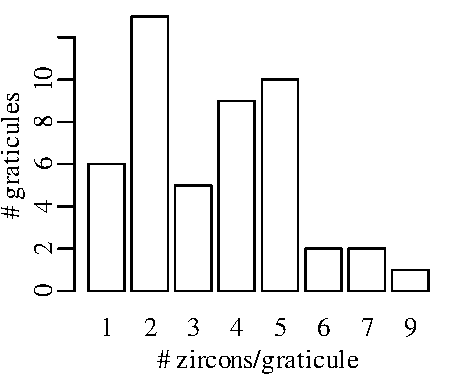
\includegraphics[width=\textwidth]{../figures/zirconhist.pdf}\medskip
\end{minipage}
\begin{minipage}[t][][t]{.7\textwidth}
  \captionof{figure}{ Histogram of the zircon counts shown in
    Figure~\ref{fig:zirconcounts}.\medskip
    ~\\
    \textbf{mean: 3.50}\\
    standard deviation: 1.85\\
    \textbf{variance: 3.40}
  }
  \label{fig:zirconhist}
\end{minipage}

Like the earthquake example, also this zircon example is characterised
by similar values for the mean and the variance. This turns out to be
a characteristic property of the Poisson distribution.

\section{Probability mass function}
\label{sec:PMF}

The Poisson distribution describes the frequency of \textit{rare
  events} in time or space.  It predicts the likelihood of observing
the number of `successes' $k$ given the long term average of successes
$\lambda$:
\begin{equation}
  P(k|\lambda) = \frac{\lambda^k e^{-\lambda}}{k!}
  \label{eq:poispmf}
\end{equation}

Thus the Poisson distribution is characterised by a single parameter,
$\lambda$. Exploring the distribution for different values of this
parameter:\medskip

\noindent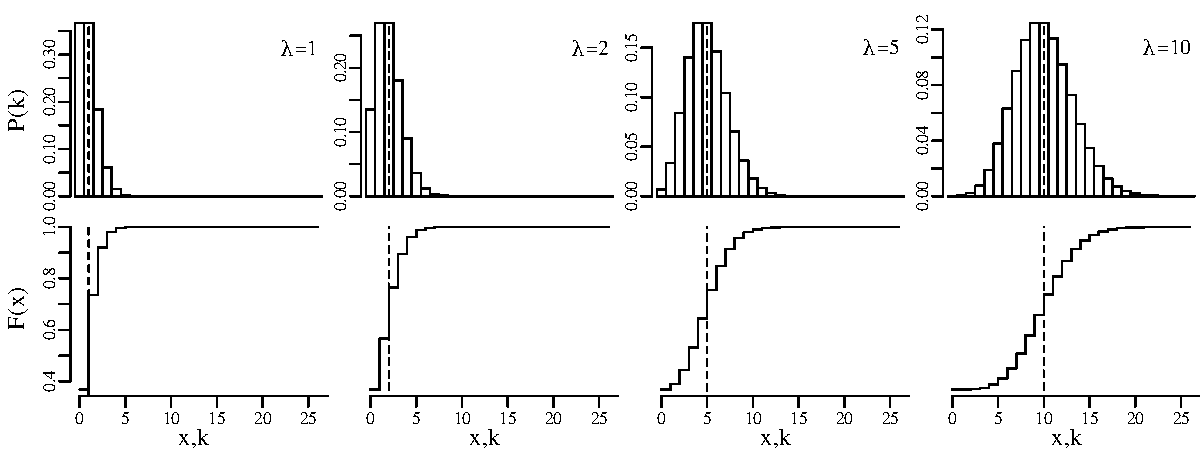
\includegraphics[width=\textwidth]{../figures/increasinglambda.pdf}
\begingroup \captionof{figure}{PMF (a -- d) and CDF (e -- h) of the
  Poisson distribution for $\lambda=1$ (a, e); $\lambda=2$ (b, f);
  $\lambda=5$ (c, g); and $\lambda=10$ (d, h); as marked by the dashed
  line.\medskip} \endgroup

The Poisson distribution is positively skewed but becomes more
symmetric with increasing $\lambda$. In this respect it is similar to
the binomial distribution (Figure~\ref{fig:binompower1}). In fact the
Poisson and binomial distributions are closely related. Recall that
the binomial distribution depends on two parameters: $n$ and $p$. It
can be shown that the binomial distribution converges to the Poisson
distribution with increasing $n$ and decreasing $p$. In the limit of
$n \rightarrow \infty$ and $p \rightarrow 0$, the binomial
distribution simplifies to a Poisson distribution with $\lambda =
{n}{p}$. The next table illustrates this by evaluating the probability
of observing $k\leq{2}$ successes under a binomial distribution with
$np=5$ for different values of $n$ and $p$:

\begin{center}
\begin{tabular}{r|llllllllll}
$n$ & 10 & 20 & 50 & 100 & 200 & 500 & 1000 & 2000 & 5000 & 10000 \\
$p$ & 0.5 & 0.25 & 0.1 & 0.05 & 0.025 & 0.01 & 0.005 & 0.0025 & 0.001 & 0.0005 \\
$P(k\leq{2})$ & 0.0547 & 0.0913 & 0.112 & 0.118 & 0.121 & 0.1234 & 0.124 & 0.1243 & 0.1245 & 0.1246
\end{tabular}
\captionof{table}{Binomial probability of 2 successes after $n$ trials
  for different values of $p$, where $np=5$. In the limit of $n
  \rightarrow{\infty}$ and $p \rightarrow{0}$, the cumulative
  probability $P(k\leq{2})$ converges to a value of 0.1246. This equals the
  probability of 2 successes under a Poisson distribution with
  $\lambda = 5$.}
\end{center}

The Poisson distribution expresses the probability of a given number
of events occurring in a fixed interval of time or space if these
events occur with a \textbf{constant mean rate} and are
\textbf{independent} of the time since the last event. Examples of
Poisson variables include the number of

\begin{enumerate}
\item people killed by lightning per year;
\item mutations in DNA per generation;
\item radioactive disintegrations per unit time;
\item mass extinctions per 100 million years.
\end{enumerate}

The number of earthquakes including aftershocks and the number of
floods per year are \emph{not} Poisson variables, because they are
clustered in time.

\section{Parameter estimation}
\label{sec:poispar}

The Poisson distribution has one unknown parameter, $\lambda$. This
parameter can be estimated using the method of maximum likelihood,
just like the parameter $p$ of the binomial distribution
(Section~\ref{sec:binompar}). As before, the likelihood function is
obtained by swapping the parameter ($\lambda$) and the data ($k$):
\begin{equation}
  \mathcal{L}(\lambda|k) = \frac{\lambda^k e^{-\lambda}}{k!}
  \label{eq:poislik}
\end{equation}

And as before, we can estimate $\lambda$ by taking the derivative of
$\mathcal{L}$ with respect to it and setting this derivative to zero:
\begin{equation}
  \frac{\partial{\mathcal{L}}}{\partial{\lambda}} = 0
\end{equation}

Alternatively, we can also maximise the \textbf{log-likelihood}:
\begin{equation}
  \mathcal{LL}(\lambda|k) = k \ln[\lambda] - \lambda - \sum\limits_{i=1}^{k}i
  \label{eq:poisLL}
\end{equation}

\noindent and set its derivative w.r.t. $\lambda$ to zero:
\begin{equation}
  \frac{\partial{\mathcal{LL}}}{\partial{\lambda}} = 0
\end{equation}

Both approaches give exactly the same result because any parameter
value $\hat{\lambda}$ that maximises $\mathcal{L}$ also maximises
$\mathcal{LL}$.  Thus:
\begin{equation}
  \left.\frac{\partial{\mathcal{LL}}}{\partial{\lambda}}\right|_{\hat{\lambda}} =
  \frac{k}{\hat{\lambda}} - 1 = 0
\end{equation}

\noindent which leads to
\begin{equation}
  \frac{k}{\hat{\lambda}} = 1
\end{equation}

\noindent and, hence
\begin{equation}
  \hat{\lambda} = k
  \label{eq:lambda=k}
\end{equation}

In other words, the measurement itself equals the `most likely'
estimate for the parameter. However the maximum likelihood estimate is
not the only option. Other values of $\lambda$ may also be compatible
with $k$, and vice versa. The next section explores which values of
$k$ are reconsilable with a given value of $\lambda$.

\section{Hypothesis tests}
\label{sec:poishyp}

Hypothesis testing for Poisson variables proceeds in exactly the same
way as for binomial variables (Section~\ref{sec:binomH}). For example:

\begin{enumerate}
\item Consider the following one-sided pair of hypotheses:

  \noindent\begin{minipage}{.4\textwidth}
    $H_0$ (\textbf{null hypothesis})
    
    \vspace{1em}
    
    $H_{\!A}$ (\textbf{alternative hypothesis}):
  \end{minipage}
  \begin{minipage}{.2\textwidth}
  \end{minipage}
  \begin{minipage}{.2\textwidth}
    $\lambda = 3.5$
    
    \vspace{1em}
    
    $\lambda>{3.5}$
  \end{minipage}
  \begin{minipage}{.2\textwidth}
  \end{minipage}\medskip

\item Like for the binomial case, the test statistic is the number of
  `successes'.  Suppose that we have observed $k=9$ successes.

\item The null distribution of the test statistic is a Poisson
  distribution with $\lambda={3.5}$:
  
  \begin{tabular}{c@{~}c@{~}c@{~}c@{~}c@{~}c@{~}c@{~}c@{~}c@{~}c@{~}c@{~}c}
    k & 0 & 1 & 2 & 3 & 4 & 5 & 6 & 7 & 8 & \textit{9} & 10 \\ \hline
    $P(T=k)$ & 0.030 & 0.106 & 0.185 & 0.216 & 0.189 &
    0.132 & 0.077 & 0.038 & 0.017 & \textit{0.007} & 0.002 \\
    $P({T}\geq{k})$ & 1.000 & 0.970 & 0.864 & 0.679 & 0.463 &
    0.275 & 0.142 & 0.065 & 0.027 & \textit{0.010} & 0.003 \\
  \end{tabular}

\item We will use the same significance level as always,
  i.e. $\alpha=0.05$.

\item Marking the rejection region in bold:

  \begin{tabular}{c@{~}c@{~}c@{~}c@{~}c@{~}c@{~}c@{~}c@{~}c@{~}c@{~}c@{~}c}
    k & 0 & 1 & 2 & 3 & 4 & 5 & 6 & 7 & \textbf{8} &
    \textbf{\textit{9}} & \textbf{10} \\ \hline
    $P(T=k)$ & 0.030 & 0.106 & 0.185 & 0.216 & 0.189 &
    0.132 & 0.077 & 0.038 & 0.017 & \textit{0.007} & 0.002 \\
    $P({T}\geq{k})$ & 1.000 & 0.970 & 0.864 & 0.679 & 0.463 &
    0.275 & 0.142 & 0.065 & \textbf{0.027} & \textbf{\textit{0.010}} &
    \textbf{0.003} \\
  \end{tabular}

\item\label{it:poisl351sided} The rejection region is $R =
  \{8,9,10,\ldots,\infty\}$, which includes our observation
  $k=9$. Therefore, our null hypothesis is rejected.

\end{enumerate}

Displaying the rejection region graphically:

\noindent\begin{minipage}[t][][b]{.6\textwidth}
  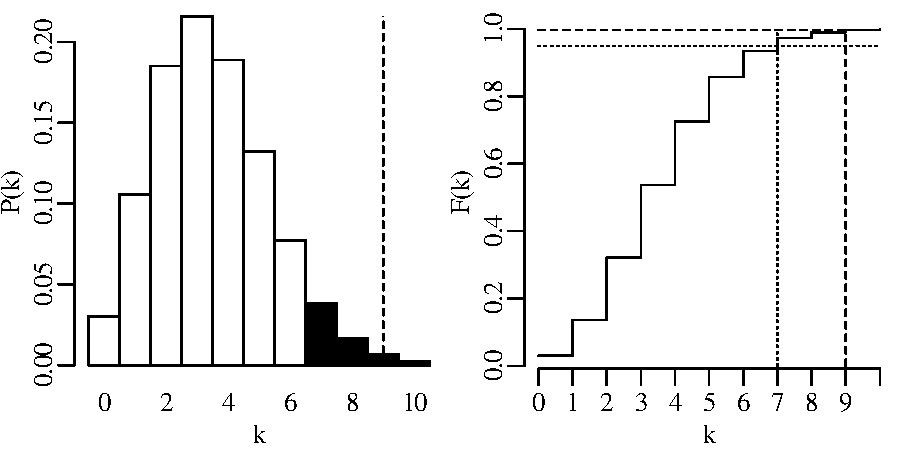
\includegraphics[width=\textwidth]{../figures/poishyp.pdf}\medskip
\end{minipage}
\begin{minipage}[t][][t]{.4\textwidth}
  \captionof{figure}{a) PMF and b) CDF of a Poissonian null
    distribution with $\lambda=3.5$. The rejection region is marked in
    black on a).  The horizontal dotted line in b) shows the
    $1-\alpha=0.95$ mark. The horizontal dashed line in the CDF marks
    the cumulative probability for $k=9$, which is greater than the
    0.95 cutoff. Therefore the one-sided null hypothesis is rejected.}
  \label{fig:poishyp}
\end{minipage}

\section{Multiple testing}
\label{sec:multipletesting}

The observant reader may have noticed that the hypothesis test of
Section~\ref{sec:poishyp} referred to the zircon counting example of
Figures~\ref{fig:zircons} -- \ref{fig:zirconcounts}. The average
number of observations per bin in this example was 3.5. And therefore,
according to Section~\ref{sec:poispar}, the maximum likelihood
estimate for $\lambda$ is 3.5 as well. According to our hypothesis
test, a value of $k=9$ is incompatible with a parameter value of
$\lambda=3.5$. Yet the observant reader may also have noticed that a
value of $k=9$ appears in the dataset
(Figure~\ref{fig:zirconcounts})!\medskip

Does this mean that our data do not follow a Poisson distribution?\medskip

The answer is no. The apparent contradiction between the
point-counting data and the hypothesis test is a result of multiple
hypothesis testing. To understand this problem, we need to go back to
the multiplicative rule of page~\pageref{page:multiplication}.  The
probability of incurring a type-I error is $\alpha$. Therefore, the
probability of not making a type-I error $1-\alpha=0.95$.  But this is
only true for one test. If we perform two tests, then the probability
of twice avoiding a type-I error is $(1-\alpha)^2=0.9025$. If we do
$N$ tests, then the probability of not making a type-I error reduces
to $(1-\alpha)^N$. Hence, the probability of making a type-I error
increases to $1-(1-\alpha)^N$. Figure~\ref{fig:zirconcounts} contains
${4}\times{12}=48$ squares. Therefore, the likelihood of a type-I
error is not $\alpha$ but $1-(1-\alpha)^{48}=0.915$.\medskip

In other words, there is a 91.5\% chance of committing a type-I error
when performing 48 simultaneous tests. One way to address this issue
is to reduce the confidence level of the hypothesis test from $\alpha$
to $\alpha/N$, where $N$ equals the number of tests.  This is called a
\textbf{Bonferroni correction}. In the case of our zircon example, the
confidence level would be reduced from $\alpha=0.05$ to
$\alpha=0.05/48=0.00104$ ($1-\alpha=0.99896$).  It turns out that the
99.896\% percentile of a Poisson distribution with parameter
$\lambda=3.5$ is 10. So the observed outcome of $k=9$ zircons in the
48 square graticule is in fact not in contradiction with the null
hypothesis, but falls within the range of expected values.\medskip

Multiple testing is a common problem in science, and a frequent source
of spurious scientific `discoveries'. For example, consider a dataset
of 50 chemical elements measured in 100 samples. Suppose that you test
the degree of correlation between each of these elements and the gold
content of the samples. Then it is inevitable that one of the elements
will yield a `statistically significant' result. Without a
multi-comparison correction, this result will likely be spurious. In
that case, repetition of the same experiment on 100 new samples would
not show the same correlation. Poorly conducted experiments of this
kind are called statistical \emph{fishing expeditions}, \emph{data
  dredging} or \emph{p-hacking}. Sadly they are quite common in the
geological literature, and it is good to keep a sceptical eye out for
them.

\section{Confidence intervals}
\label{sec:poisCI}

The construction of confidence intervals for the Poisson parameter
$\lambda$ proceeds in pretty much the same way as it did for the
binomial parameter $p$. Let us construct a 95\% confidence interval
for $\lambda$ given the observation that 5 magnitude 5.0 or greater
earthquakes occurred in the US in 2016.\medskip

The lower limit of a 95\% confidence interval for the number of
earthquakes per year is marked by the value of $\lambda$ that is more
than 2.5\% likely to produce an observation of $k=5$ or greater. This
turns out to be $\lambda=1.62$. The upper limit of the confidence
interval is marked by the value of $\lambda$ that is more than 97.5\%
likely to produce an observation of $k=5$ or smaller. This value is
$\lambda=11.7$. Hence, 95\% confidence interval is $[1.62, 11.7]$.
Note that this interval includes the average of all 100 preceding
years. \medskip

\noindent\begin{minipage}[t][][b]{.6\textwidth}
  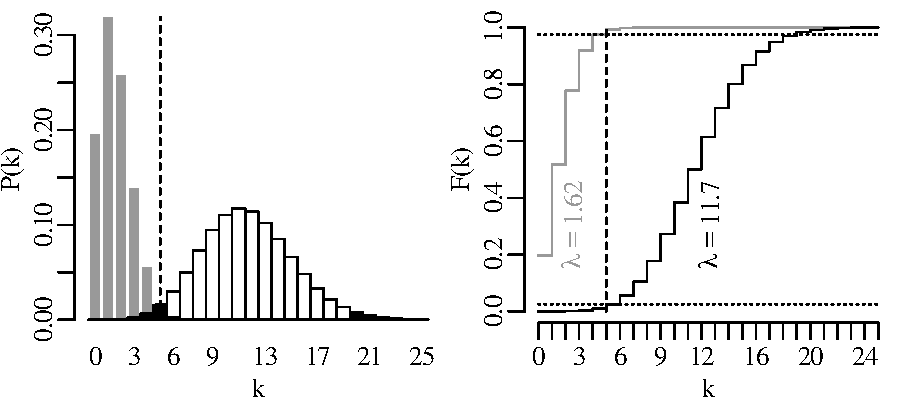
\includegraphics[width=\textwidth]{../figures/poisci.pdf}\medskip
\end{minipage}
\begin{minipage}[t][][t]{.4\textwidth}
  \captionof{figure}{95\% confidence interval for the Poisson
    parameter $\lambda$ given a single observation of $k=5$ events.
    The lower ($p=1.62$, grey) and upper ($p=11.67$) limits of the
    confidence interval are shown as a) PMFs and c) CDFs. Dotted
    horizontal lines mark the 0.025 and 0.975 confidence levels.}
  \label{fig:poisci}
\end{minipage}

Repeating the exercise for all observations in
Figure~\ref{fig:declusteredquakes} yields the following set of 100
confidence intervals for $\lambda$:\medskip

\noindent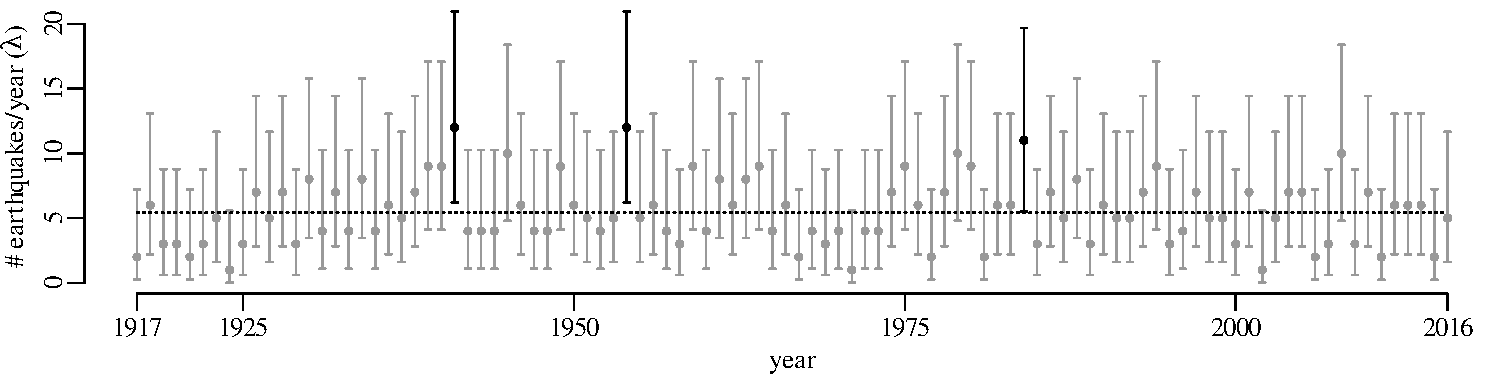
\includegraphics[width=\textwidth]{../figures/poiserrbars.pdf}
\begingroup \captionof{figure}{95\% Poisson confidence intervals for
  all the years in the declustered earthquake database. The horizontal
  dotted line marks the average of all the years
  ($\hat{\lambda}=5.43$). `outliers' are marked in black.\medskip}
\endgroup

Three years (1941, 1954 and 1984) stand out because their 95\%
confidence intervals do not overlap with the long term average value
of 5.43. Does this mean that the earthquake statistics did not fit the
Poisson distribution during those years? The answer to this question
is no, for the same reasons as given in
Section~\ref{sec:multipletesting}. When a large number of confidence
intervals are drawn, it is inevitable that some of these do not
include with the true parameter value. In fact it would be suspicious
if all the error bars overlapped with the long term average.\medskip

With a confidence level of $\alpha=0.05$, there should be a 5\%
chance of committing a type-I error.  Therefore, we would expect 5\%
of the samples to be rejected, and 5\% of the error bars to exclude
the true parameter value. The observed number of rejected samples
(3/100) is in line with those expectations.
